
\setchapterimage[6cm]{cabecera3}
\setchapterpreamble[u]{\margintoc}
%%%%%%%%%%%%%%%%%%%%%%%%%%%%%%%%%%%%%%%%%%%%%%%%%%%%%%%%%%%%%

\chapter{Comunicación Indirecta }
\label{ch:Comunicación Indirecta}
\index{comunicación indirecta}

En \gls{comunicacion indirecta}  la naturaleza  del intermediario  y del acoplamiento  varían de un enfoque a otro y entre sistemas:  se puede establecer  conceptos de acoplamiento tanto temporal como espacial que determinan como el receptor y el emisor coinciden o no en el tiempo y en espacio.

En la tabla \ref{tab:acopla} se plasman las posibles variantes en este tipo de enfoque. Por ejemplo, las técnicas consideradas hasta ahora se basan en un acoplamiento directo o sistemas \gls{fuertemente acoplado}, como las arquitecturas clientes-servidor. Son arquitecturas acopladas en tiempo y espacio.
Por otra parte, las aplicaciones como el correo electro\'onico, son arquitecturas  desacopladas  en tiempo y  acopladas en espacio, ver descripci\'on en la parte superior, derecha de la tabla \ref{tab:acopla}.

 Mientras que la multidifusi\'on puede catalogarse como arquitecturas acoplada en tiempo, desacopladas en espacio, descrita en la parte inferior e izquierda de la tabla \ref{tab:acopla}.
Y las arquitecturas que calzan en la categor\'ia  de desacoplamiento en espacio y tiempo, como las arquitecturas Pub-sub y colas de mensajes, ubicada en la parte inferior, derecha.
 
 
%%%%%%%%%%%%%%%%%%%%%%%
%\marginnote[4cm]{
	\begin{kaobox}[frametitle=Acoplamiento]
	  El concepto de Acoplamiento propuesto por Yourdon y Constantine  en su libro, Structured Design: Fundamentals of a Discipline of Computer Program and Systems Design, \cite{Yourdon1979}	
\end{kaobox} %%  }
%%%%%%%%%%%%%%%%%%

\definecolor{LightCyan}{rgb}{0.88,1,1}
\begin{table}[h]\index{acoplamiento en espacio y tiempo}
	\footnotesize%
	\begin{center}
	\footnotesize
     \begin{tabular}{p{0.2\textwidth}p{0.35\textwidth}p{0.35\textwidth}}
			\toprule
		   	  & \cellcolor{LightCyan} Acoplado en tiempo  & \cellcolor{LightCyan} Desacoplado  en tiempo\\
		    \midrule
		   
			\quad  \cellcolor{LightCyan} Acoplado en espacio  & Comunicación dirigida a un receptor o a varios receptores de un mensaje. Los receptores deben existir en ese momento del tiempo. &  Comunicación dirigida a un receptor(es) de un mensaje. Receptores o emisores pueden no existir en ese momento del tiempo.\\  			
					\\
			\quad \cellcolor{LightCyan} Des acoplado en espacio  & Emisor no necesita saber la identidad del receptor o receptores. Emisor y receptor deben existir al mismo tiempo. & Emisor no necesita saber la identidad del receptor o receptores. Los receptores o emisores pueden no existir en ese momento del tiempo.  \\
		 	 
			\addlinespace 
			\bottomrule
		
		\end{tabular}
	\end{center}
	\caption{Acoplamiento en Espacio y Tiempo.  Adaptado de \CO }
	\label{tab:acopla}
\end{table}
%%%%%%%%%

En lo que sigue, se estudian algunas de las arquitecturas de comunicaci\'on indirecta: Grupos, pub-sub y colas.

%%%%%%%%%%%%%%%%%%%%%%%%%%%%%%%%%%%%%%%%%%%%%%%%%%%%%%%%%%%%%
\section{Grupos}
\index{grupos}

La \gls{comunicacion grupal}   es una abstracción sobre la comunicación de multidifusión y se puede implementar a través de multidifusión IP o una red de superposición equivalente, teniendo como valor adicional  la  gestión de pertenencia al grupo, detección de fallas y garantía de confiabilidad y pedidos, \cite{Verissimo2012}, \cite{Coulouris2011}.

\subsection{Modelo de Programaci\'on}  
\index{modelo de programaci\'on de grupos}

En la comunicación grupal, el concepto central es el de un \textbf{grupo} con una \textbf{membresía de grupo} asociada y  con los procesos  de \textbf{unirse} o \textbf{salir} del grupo ver figura \ref{fig:modeloprog-group}. Los procesos pueden enviar un mensaje a este grupo y hacer que se propague a todos los miembros (o a un miembro) del grupo con ciertas garantías en términos de confiabilidad y orden. Así, la comunicación de grupo implementa la \gls{comunicacion multidifusion}, as\'i como tambi\'en la \gls{comunicacion unidifusion}. 

\begin{figure}%
	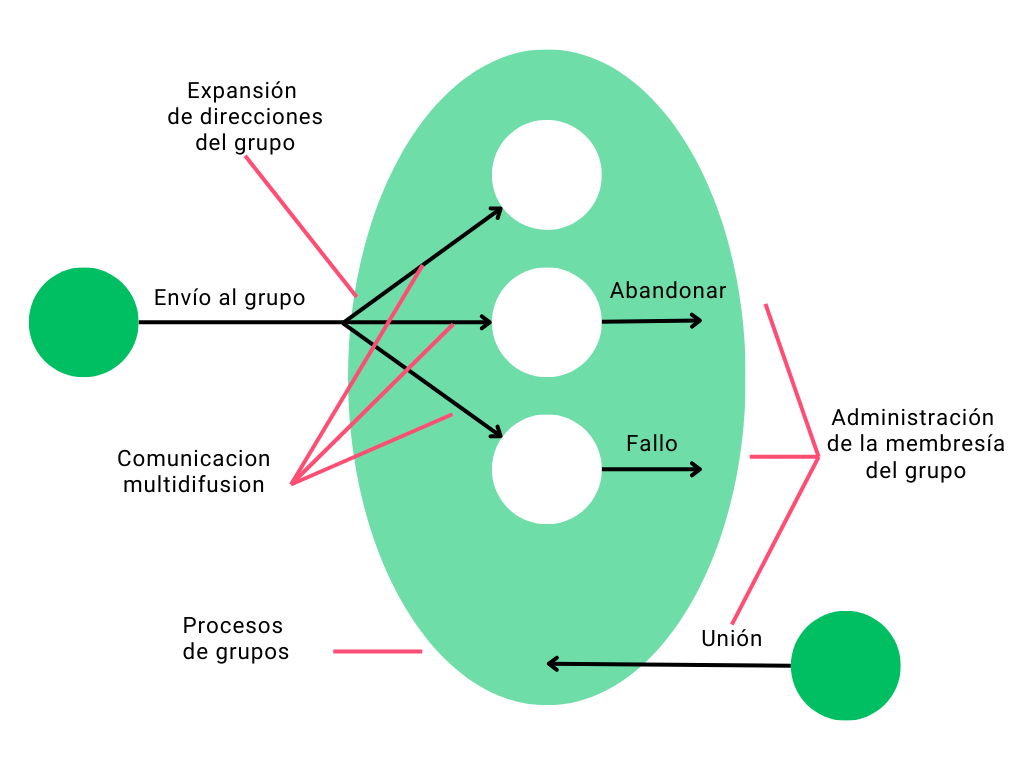
\includegraphics{6/modeloprogramacion.png}
	\caption{Model de Programaci\'on. Tomado de \cite{Coulouris2011}}
	\label{fig:modeloprog-group}
\end{figure}

El uso de una única operación de envío permite  un uso   eficiente del ancho de banda. También es relevante en términos de garantías de entrega del mensaje ya que la operci\'on de env\'io del mensaje se asocia a un proceso. Si ocurre una falla y alg\'un mensaje no se entrega, se puede implementar el reenvio de mensajes.

\subsection{Membres\'ia del Grupo}

Un servicio de membresía grupal tiene cuatro tareas principales: \index{membres\'ia de grupos}

\begin{description}
	\item[Interfaz para cambios de membresía de grupo]: el servicio de membresía proporciona operaciones para crear/destruir grupos de procesos y para agregar/retirar un proceso hacia o desde un grupo. En la mayoría de los sistemas, un solo proceso puede pertenecer a varios grupos al mismo tiempo (grupos superpuestos ).  
	
	\item[Detección de fallas]: el servicio monitorea a los miembros del grupo no solo en caso de que se bloqueen, sino también en caso de que se vuelvan inaccesibles debido a una falla de comunicación. El detector marca los procesos como sospechosos o no sospechosos. El servicio utiliza el detector de fallas para tomar una decisión sobre la situación de la membresía del grupo: excluye un proceso de la membresía si se sospecha que ha fallado 	o si se ha vuelto inalcanzable.
	
	\item[Notificación de cambios en la membresía del grupo]:  el servicio notifica al los miembros del grupo  cuando se agrega un proceso, o cuando se excluye un proceso (por falla o 	cuando el proceso se retira deliberadamente del grupo).
	
	\item[Difusión de direcciones de grupo]: cuando un proceso difunde un mensaje en forma múltiple, proporciona el identificador de grupo en lugar de una lista de procesos del grupo. El servicio de administración de membresía expande el identificador a la membresía del grupo actual para su entrega. El servicio puede coordinar la entrega de multidifusión con cambios de membresía controlando la expansión de direcciones. Es decir, puede decidir sistemáticamente dónde enviar un mensaje determinado, aunque la membresía pueda cambiar durante la entrega.
	
\end{description}

\subsection{Caracter\'isticas de la arquitectura de Grupos}
\index{procesos en grupos} \index{objetos en grupos}
\index{grupos abiertos} \index{grupos cerrados}
\index{grupos superpuestos} \index{grupos no superpuestos}

\begin{description}
	\item[Grupos de procesos] La mayor parte del trabajo en servicios grupales se centra en  grupos donde las entidades comunicantes son Procesos. El nivel de servicio proporcionado por los grupos de procesos es similar al de los sockets.
	\item[Grupos de objetos]  Es una colección de objetos (instancias de la misma clase) que procesan el mismo conjunto de invocaciones al mismo tiempo, y cada una devuelve respuestas. Los clientes invocan operaciones en un único objeto local, que actúa como proxy del grupo. El proxy utiliza un sistema de comunicación grupal para enviar las invocaciones a los miembros del grupo de objetos. Los parámetros de objeto y los resultados se empaquetan como en RMI y las llamadas asociadas se envían automáticamente a los objetos/métodos de destino.
	
	\item[Grupos abiertos] Un grupo está abierto si los procesos fuera del grupo pueden enviarle mensajes, figura \ref{fig:grupo-abcerr}. Los grupos abiertos son útiles, por ejemplo, para entregar mensajes a grupos de procesos interesados.  
	
	\item[Grupos cerrados]  Se dice que el grupo está cerrado si solo los miembros del grupo pueden enviar mensajes  multidifusión. Un proceso en un grupo cerrado se entrega a sí mismo cualquier mensaje que difunde al grupo, ver  figura \ref{fig:grupo-abcerr}. Los grupos cerrados de procesos son útiles, por ejemplo, para servidores que cooperan para enviarse mensajes entre sí que solo ellos deberían recibir.
	
	\item[Grupos Superpuestos]  Entidades (procesos u objetos) pueden ser miembros de varios grupos
	
	\item[Grupos no Superpuestos] Implican que la membresía no se superpone (es decir, cualquier proceso pertenece como máximo a un grupo)
	
\end{description}
 
	\begin{figure}%
		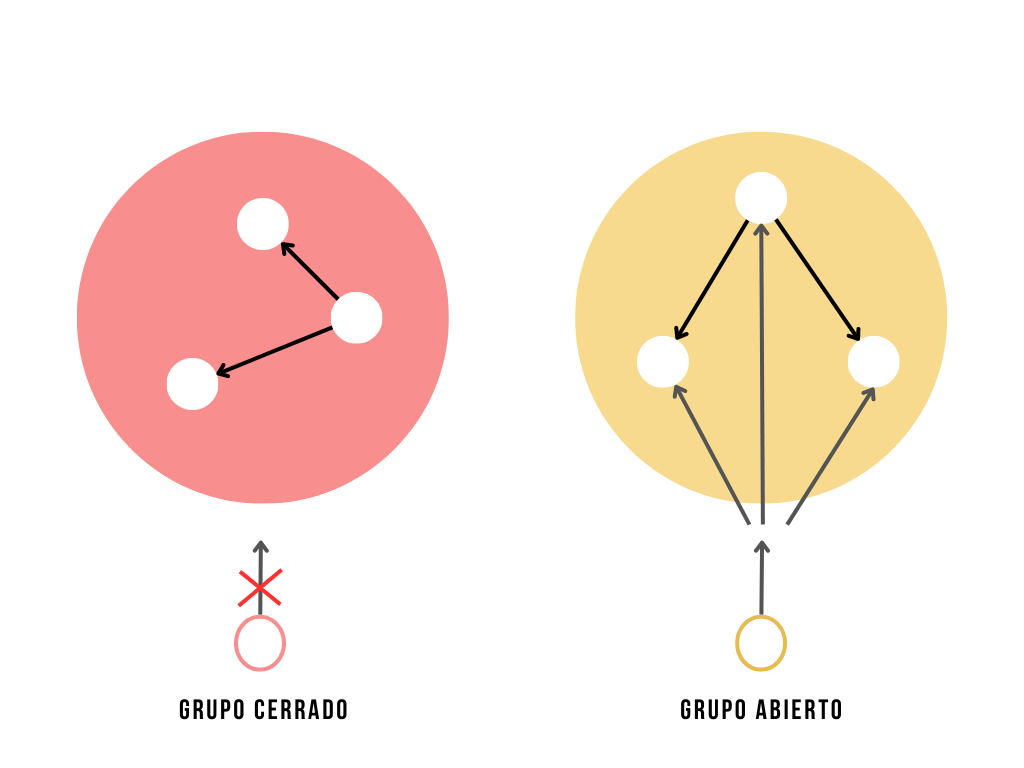
\includegraphics{6/abierto-cerrado.png}
		\caption{Grupos cerrados y abiertos. Tomado de \cite{Coulouris2011}}
		\label{fig:grupo-abcerr}
	\end{figure}
%%%%%%%%%%%%%%%%%%%%%%%%%%%%%%%%%%%%%%%%%%%%%%%%%%%%%%%5	

\subsection{Confiabilidad y ordenamiento en multidifusi\'on}
Otras caracter\'isticas atribuida a los grupos esta la confiabilidad y el ordenamiento de los mensajes.

\paragraph{Confiabiliad}
\index{confiabilidad en grupos}
La confiabilidad en la comunicación  se ha definido   en términos de las siguientes propiedades:
 
	\begin{description}
		\item [Integridad] El mensaje recibido es el mismo que el enviado, y no se entregan dos veces.
		\item [Validez] Cualquier mensaje saliente es eventualmente entregado. La interpretación de multidifusión confiable se basa en estas propiedades, con integridad definida  en términos de entregar el mensaje correctamente como máximo una vez, y la validez interpretado como que garantiza que un mensaje enviado finalmente será entregado.
		\item [Acuerdo]  Para extender la semántica y cubrir la entrega a múltiples receptores, la propiedad \textit{acuerdo} indica que si el mensaje se entrega a un proceso, entonces se entrega a todos los procesos del grupo.
	\end{description} 

\paragraph{Ordenamiento}
\index{ordenamiento en grupos}
Además de las garantías de fiabilidad, la comunicación grupal exige garantías adicionales en términos del orden relativo de los mensajes entregados a múltiples destinos.   Para contrarrestar los retrasos y desorden en la entrega, los servicios de comunicación grupal ofrecen multidifusión ordenada, con la opción de una o más de las siguientes propiedades:
\begin{description}
	\item[Orden FIFO]: ordenamiento primero en entrar, primero en salir (FIFO)  se ocupa de preservar el pedido desde la perspectiva del remitente del 	proceso, en el sentido de que si un proceso envía un mensaje antes que otro, se entregará en este orden en todos los procesos del grupo.
	
	\item[Ordenamiento causal]: el ordenamiento causal tiene en cuenta las relaciones causales entre mensajes, en el sentido de que si un mensaje ocurre antes que otro mensaje en el sistema distribuido,  esta   relación causal se conservará en la entrega de los mensajes asociados en todos los procesos  
	\item[Ordenamiento total]: En el orden total, si un mensaje se entrega antes que otro mensaje en un proceso, se conservará el mismo orden en todos los procesos.
\end{description}

%%%%%%%%%%%%%%%%%%%%%%%%%%%%%%%%%%%%%%%%%%%%%%%%%%%
%%%%%%%%%%%%%%%%%%%%%%%%%%%%%%%%%%%%%%%%%%%%%%%%%%%
\section{Publicaci\'on-Suscripci\'on}
\label{sec:pubsub}
\index{pub-sub}
Las principales entidades en un sistema \gls{pub-sub}  son los \textbf{editores} y \textbf{suscriptores} de contenido \sidecite{Tarkoma2012}. Un \textbf{publicador} (\textit{publisher}) detecta un evento y luego lo publica en forma de notificación.
Una \textbf{notificación} encapsula información relacionada con el evento observado. La notificación  denota que ha ocurrido un evento observado.
Un \textbf{evento} representa cualquier transición de estado discreta que ha ocurrido y se señala desde una entidad a un número de otras entidades.

Un \textbf{suscriptor}, por ejemplo, podría expresar interés en todos los eventos relacionados con este libro de texto, como la disponibilidad de una nueva edición o actualizaciones del sitio web relacionado. La tarea del sistema de publicación y suscripción es hacer coincidir las suscripciones con los eventos publicados y garantizar la entrega correcta de las notificaciones de eventos. Un evento dado se entregará potencialmente a muchos suscriptores y, por lo tanto, en  publicación y suscripción  se usan   paradigmas de comunicaciones de uno a muchos.

%%%%%%%%%%%%%%%%%%%%%%%%%%%%%%%%%%%%%%%%%%%%
\subsection{Aplicaciones de los sistemas de publicación-suscripción}  
\index{aplicaciones pub-sub }  
Los sistemas de publicación-suscripción se utilizan en una  variedad de dominios de aplicación, en particular los relacionados con la difusión de eventos a gran escala.   Ejemplos  incluyen \sidecite{Tarkoma2012}:
\begin{itemize}
	\item 	\textbf{GUI}, en las que los sistemas pub/sub se aplica como el pegamento que conecta los diversos componentes entre sí. Un ejemplo  es el patrón de diseño \textbf{MVC} (Modelo Vista Controlador) muy utilizado en 	GUIs y su componente el patrón de observador. 
	\item Push de información, en el que se publica el contenido al usuario. Este es un requisito  para  aplicaciones que dependen de datos en tiempo real o casi en tiempo real.
	\item  Filtrado de información y entrega dirigida utilizada por los servicios de alerta y presencia (Google Alerts, etc.), tiendas de aplicaciones, servicios de corretaje de RSS, etc. Los ejemplos incluyen \textbf{XMPP Pub/sub}, \textbf{Pubsubhubbub}, \textbf{Facebook Messenger and Chat }y \textbf{Twitter}.
	\item Plano de señalización, en el que pub/sub asegura que los eventos asíncronos se entregan en 	en tiempo real o casi en tiempo real desde la publicación de componentes hasta la suscripción de componentes.
	Las aplicaciones de ejemplo incluyen sistemas industriales y tácticos. DDS (Data Distribution Systems) es el estándar clave 	para estos sistemas.
	\item La arquitectura orientada a servicios (SOA) y las aplicaciones comerciales se basan en publicación/suscripción en el bus de servicios empresariales (ESB). El ESB normalmente se implementa con un \textit{broker} de mensaje XML.
	\item Procesamiento de Eventos Complejos (CEP) para análisis de datos. CEP se utiliza ampliamente en varios 	aplicaciones comerciales, por ejemplo, comercio algorítmico y detección de fallas.
	\item Computación en la nube, en la que pub/sub y colas de mensajes se utilizan para conectar los  componentes de la nube.
	\item Internet de las cosas, en el que pub/sub conecta los sensores y actuadores entre sí 	con recursos de Internet.
	\item Juegos multijugador en línea, en los que pub/sub se usa para sincronizar el estado del juego en jugadores y servidores

\end{itemize}
 

%%%%%%%%%%%%%%%%%%%%%%%%%%%%%%%%%%%%%%%%%%%%%%%

\subsection{Modelo de Programaci\'on}
\index{modelo de programaci\'on pub-sub}

El modelo de programación en los sistemas de publicación-suscripción se basa en un pequeño conjunto de operaciones, ver Figura \ref{fig:paradigma}. Los editores difunden un evento $e$ a través de una operación de $publicacion(e)$ y los suscriptores expresan su interés en un conjunto de eventos a través de suscripciones. En particular, logran esto a través de una operación de $suscripcion(f)$ donde f se refiere a un filtro, es decir, un patrón definido sobre el conjunto de todos los eventos posibles.

 La expresividad de los filtros  está determinada por modelo de la suscripción. Los suscriptores pueden revocar este interés mediante la correspondiente operación de $cancelacion-suscripcion(f)$. Cuando los eventos llegan a un suscriptor, los eventos se entregan usando una operación de $notificacion(e)$.

Algunos sistemas complementan el conjunto de operaciones  anuncios. Con los anuncios, los editores tienen la opción de declarar la naturaleza de los eventos futuros a través de una operación de $anuncios(f)$. 

\begin{figure}%
	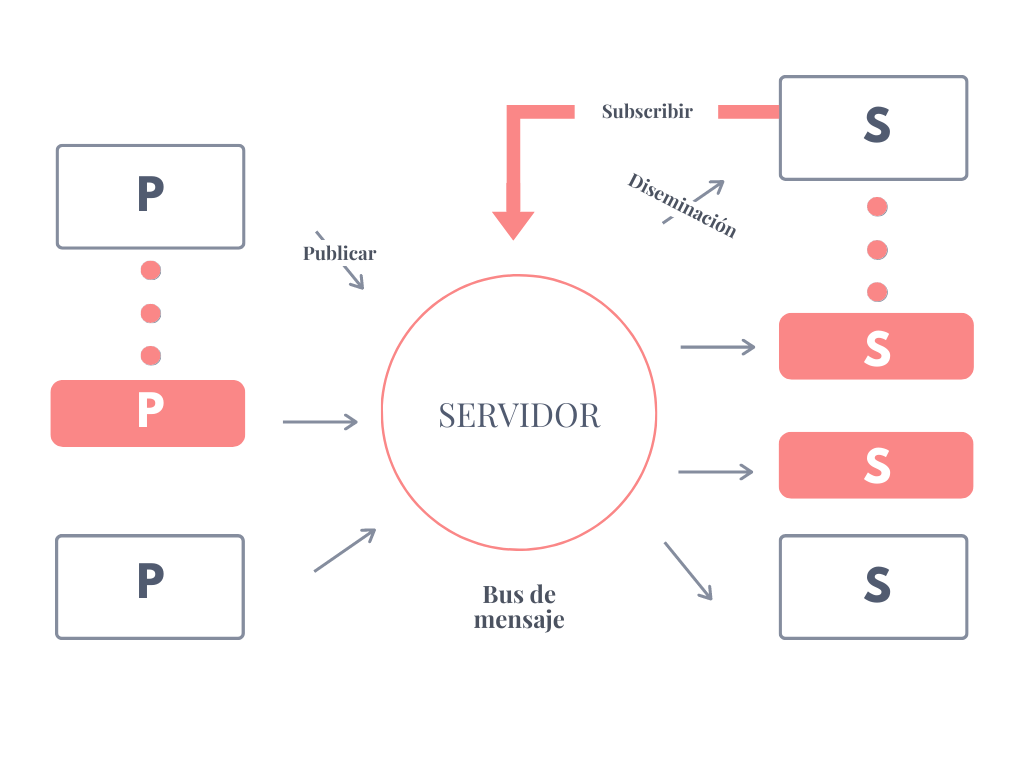
\includegraphics {6/pub-sub.png}
	\caption{Paradigma Publicaci\'on Suscripci\'on.}
	\label{fig:paradigma}
\end{figure}

 \paragraph{Modelo de Subscripci\'on}
\index{modelo de subscripci\'on  pub-sub} 

La expresividad de los sistemas de publicación-suscripción está determinada por el\textbf{ modelo de suscripción}, que cuentan con una serie de esquemas o filtros \sidecite{Tarkoma2012} \sidecite{Coulouris2011}:

\begin{description} 
	
	\item[Basado en canales]: en este enfoque, los editores publican eventos en canales con nombre y los suscriptores luego se suscriben a uno de estos canales  para recibir todos los eventos enviados a ese canal. Este   esquema  es el \'unico que se define en un canal físico.
	
	\item[Basado en temas]: se  asume que cada notificación se expresa en términos de varios campos, con un campo que denota el tema. Las suscripciones se definen en función del tema de inter\'es. Este enfoque es equivalente a los enfoques basados en canales con la diferencia de que los temas se definen implícitamente, pero se declaran como parte de un campo en el enfoque basados en temas.  
	
	\item[Basado en contenidos]:  son una generalización de enfoques basados en temas que permiten la expresión de suscripciones en una variedad de campos en solo una notificación del evento. Más específicamente, un filtro basado en contenido es una consulta definida en términos de composiciones de restricciones sobre los valores de los atributos del evento. Por ejemplo, un suscriptor podría expresar interés en eventos relacionados con el tema de los sistemas de publicación-suscripción, donde el sistema en cuestión es el \textit{Servicio de eventos CORBA} y el autor es \textit{Tim Kindberg} o \textit{Gordon Blair}. 
	
	\item[Basado en tipo]: las suscripciones se definen en términos de tipos de eventos y la coincidencia se define en términos de tipos o subtipos del filtro dado. Este enfoque puede expresar una variedad de filtros, desde un filtrado basado en nombres de tipo generales hasta consultas más detalladas que definen atributos y métodos de un objeto dado. Estos filtros detallados son similares en expresividad a los enfoques basados en contenido. %Las ventajas de los enfoques basados en tipos es que pueden integrarse en lenguajes de programación y pueden verificar la corrección del tipo de las suscripciones, eliminando algunos tipos de errores de suscripción.	
	
\end{description}


\subsection{Consideraciones de Implementaci\'on}

\paragraph{Implementaciones Centralizadas}
\index{implementaci\'on centralizada en pub-sub} 

El procesamiento de eventos y notificaciones se puede implementar fácilmente en editores y con un intermediario centralizado, ver figura \ref{fig:pub-sub1}.

En la implementaci\'on centralizada,  ocurre que: 

\begin{itemize}
	\item El enfoque más simple es centralizar la implementación en un solo nodo con un servidor en ese nodo que actúa como un intermediario de eventos.
	\item Los publicadores  publican eventos y (opcionalmente) envían anuncios al corredor, y los suscriptores envían suscripciones al corredor y reciben notificaciones a cambio.
	\item La interacción con el corredor se realiza a través de una serie de mensajes punto a punto; esto se puede implementar mediante el paso de mensajes o la invocación remota.
\end{itemize}
Este enfoque es sencillo de implementar, pero el diseño carece de resiliencia y escalabilidad, ya que el nodo  centralizado representa un punto único de posibles fallas del sistema y un cuello de botella para el rendimiento. 

\begin{figure}%
		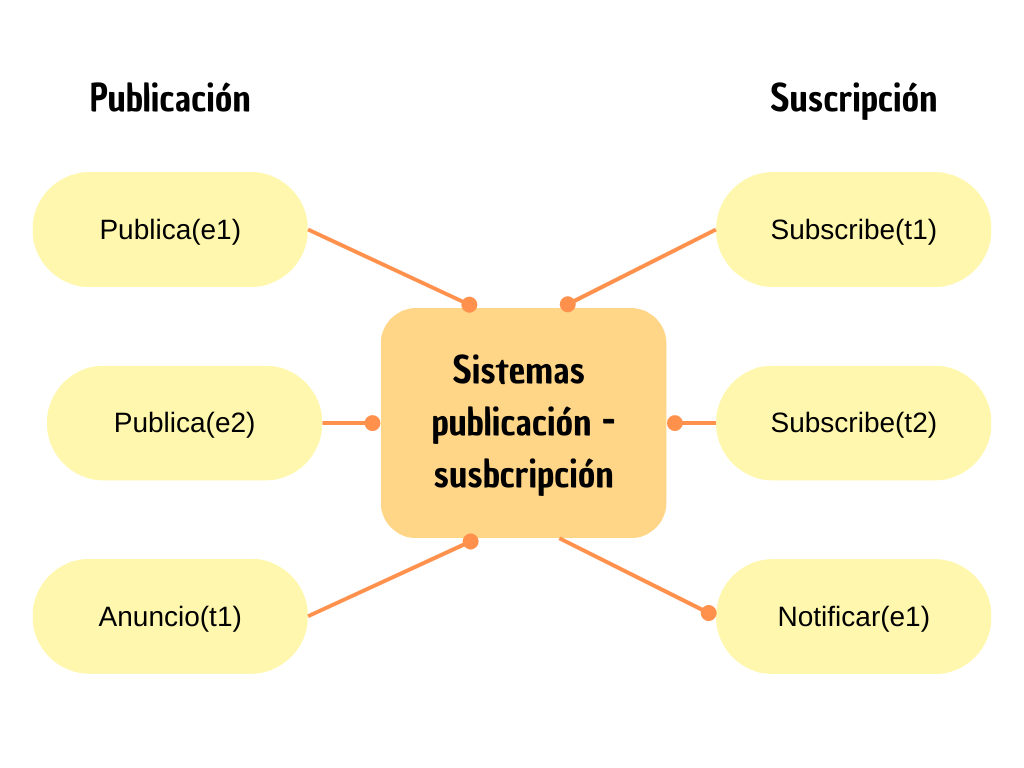
\includegraphics{6/modprog-pubsub.png}
	\caption{Publicaci\'on-Susbcripci\'on centralizado.}
	\label{fig:pub-sub1}
\end{figure}

\paragraph{Implementaciones Distribuidas}
\index{ implementaci\'on distribuida en pub-sub} 

En este esquemas, el nodo centralizado es reemplazado por una red de corredores que cooperan para ofrecer la funcionalidad deseada. 
En la visi\'on distribuida, el sistema pub-sub distribuido se implementa como una red de intermediarios o enrutadores en la  capa de aplicación que se comunican  mediante el uso de las primitivas de capa inferior, normalmente TCP/IP. En la figura \ref{fig:pub-sub2} se esquematiza una red pub-sub distribuida donde cada componente de la red de corredores son componentes intermediarios o enrutadores.

\begin{figure}%
		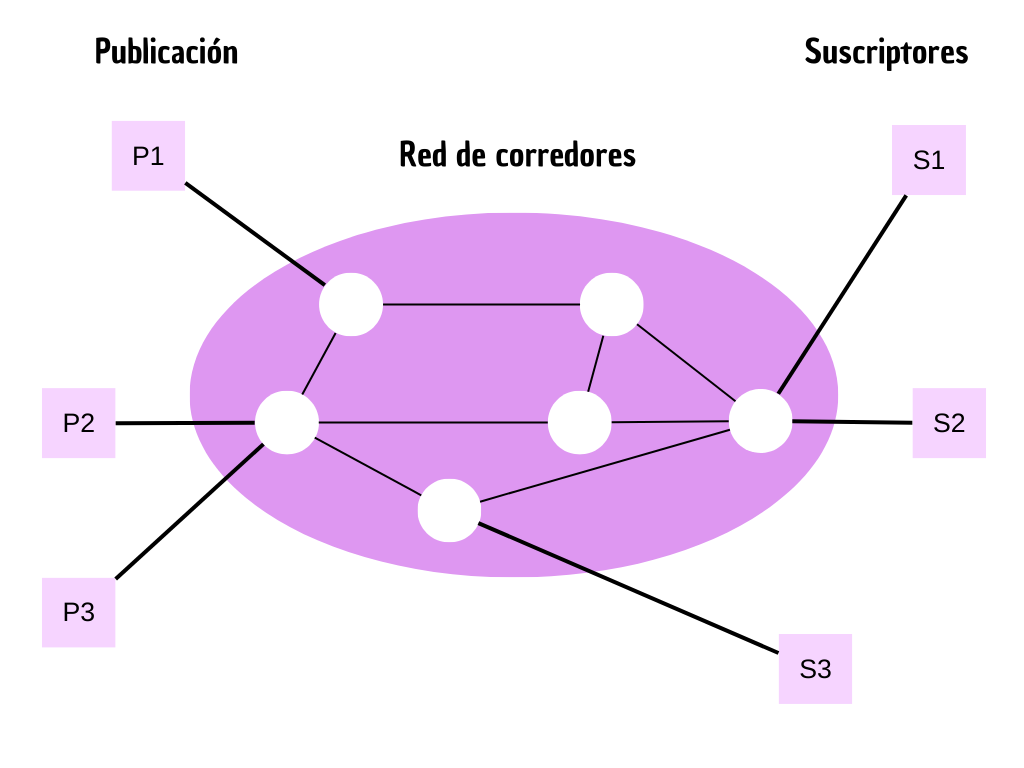
\includegraphics{6/modprog-pubsub2.png}
	\caption{Publicaci\'on-Susbcripci\'on distribuido. Tomado de \CO}
	\label{fig:pub-sub2}
\end{figure}

Dicho enfoque tienen el potencial de sobrevivir a las fallas de los nodos y se ha demostrado que pueden funcionar bien en implementaciones a escala de Internet.
Como alternativa, es posible tener una implementación completamente nodo-a-nodo \textit{(peer-to-peer)} de un sistema de publicación-suscripción.  En este enfoque, no hay distinción entre editores, suscriptores y corredores; todos los nodos actúan como intermediarios, implementando de manera cooperativa la funcionalidad de enrutamiento de los  eventos requeridos

%% \subsection*{Modelo de servicios Pub-Sub}
%%\index{Publicaci\'on-Suscripci\'on!modelo de servicio} 

%% La Figura \ref{fig:pub-sub-mod-ser} ilustra un diseño genérico de servicio pub/sub. En la figura, el servicio pub/sub  es un servicio lógicamente centralizado que proporciona las funciones e interfaces necesarias para admitir la entrega de notificaciones de los editores a los suscriptores. El servicio pub/sub  consta de los siguientes componentes clave \sidecite{Tarkoma2012}:
 
%% \begin{itemize} 	\item Un motor de notificación que construye y mantiene una estructura de índice de las suscripciones,  y utiliza una tabla de índice para reenviar notificaciones a los suscriptores. El motor ofrece las interfaces necesarias para suscriptores y editores que les permitan suscribirse, 	darse de baja y publicar contenido.
	%%	\item Un administrador de suscripciones que acepta suscripciones del motor y las mantiene. 	Las dos operaciones obligatorias son insertar y eliminar una suscripción.   	\item  Un almacenamiento de suscripciones que almacena suscripciones y datos relacionados con las suscripciones.   	\item Un almacenamiento de eventos es una instalación para almacenar eventos publicados para que puedan recuperarse  	más tarde.    	\item Un consumidor de notificación que es un componente intermediario en el proceso de notificación. Un consumidor recibe notificaciones del motor y luego las reenvía al suscriptor correspondiente. El consumidor puede almacenar, comprimir y procesar notificaciones antes de la entrega final.
 %% \end{itemize}
 
 

%%Un editor observa una situación y cuando se observa un evento de interés, una notificación se crea y se envía al motor de notificación utilizando su interfaz de publicación. La notificación luego se compara con el índice de suscripción mantenido por el motor con la ayuda de el administrador de suscripciones. El motor envía la notificación a los consumidores de notificaciones. de suscriptores que han manifestado interés en la notificación. En otras palabras, la notificación coincide con las suscripciones de los suscriptores. A continuación, se prepara la notificación. por cada consumidor para su entrega al suscriptor asociado.


%%Este modelo de servicio pub/sub separa la gestión de las suscripciones, el proceso de emparejamiento con el motor de notificaciones y la entrega final a los suscriptores. Esta separación permite, por ejemplo, cambiar de consumidor de notificación sin cambiar el motor. El diseño de la Figura \ref{fig:pub-sub-mod-ser} está lógicamente centralizado y oculta la distribución de los componentes Es necesario distribuir y replicar los componentes para lograr escalabilidad y confiabilidad en un entorno distribuido.


\subsubsection{Enfoques de Implementaci\'on} 
Existe una  variedad de enfoques de implementación  \sidecite{Tarkoma2012} \sidecite{Coulouris2011}:

\begin{description} \index{algoritmo de inundaci\'on}  \label{alg-inun}
	
	\item[Inundaci\'on (Flooding)]  el enfoque más simple se basa en Inundaci\'on. Opera de la siguiente manera:
	\begin{itemize}
		\item Se envia una notificación de evento a todos los nodos de la red y luego se realiza el emparejamiento  con el suscriptor del evento.
		\item Como alternativa, la inundación se puede utilizar para enviar suscripciones a todos los posibles publicadores;  la coincidencia se realiza en el  publicador y los eventos coincidentes se envian directamente a los suscriptores relevantes mediante la comunicación punto a punto.  La inundación se puede implementar utilizando una función de difusión o multidifusión subyacente.
		\item  Alternativamente, los intermediarios pueden organizarse en un gráfico acíclico en el que cada uno envía notificaciones de eventos entrantes a todos sus vecinos. Este enfoque tiene el beneficio de la simplicidad, pero puede resultar en una gran cantidad innecesaria de tráfico de red. 
	\end{itemize} 
	
	\item[Filtrado]: Se conoce como enrutamiento basado en filtrado. Los corredores envían notificaciones a través de la red solo donde hay una ruta a un suscriptor válido. Funciona as\'i: \index{ algoritmo de filtrado} 
	
	\begin{itemize}
		\item La propagación de la información de suscripción se realiza a través de la red hacia los editores potenciales y luego se almacena el estado asociado en cada corredor.
		\item  Específicamente, cada nodo debe mantener una \textbf{lista de vecinos} que contenga a todos los vecinos conectados en la red de corredores, una \textbf{lista de suscripción} que contenga  todos los suscriptores conectados directamente atendidos por este nodo, y una \textbf{tabla de enrutamiento}. Esta tabla de enrutamiento mantiene una lista de vecinos y suscripciones válidas para ese camino.
		
		\item Este enfoque   exige una implementación de la coincidencia en cada nodo en la red de corredores: en particular, en la función de coincidencia lleva a cabo la notificación de eventos y una lista de nodo junto con la suscripción y las devoluciones asociadas en el conjunto de nodos donde la notificación coincide con la suscripción.
	\end{itemize}
	El algoritmo específico para este enfoque de filtrado se captura en las Figura \ref{fig:filtrado} y opera de la siguiente manera:
	
	\begin{figure}
		\centering
		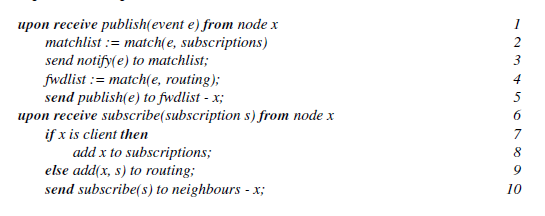
\includegraphics{6/Filtrado.png}
		\caption{Algoritmo de Filtrado. Tomado de \CO}
		\label{fig:filtrado}
	\end{figure}
	
	
	\begin{itemize}
		\item  Cuando un corredor recibe en la solicitud de publicación de un nodo dado, debe pasar esta notificación a todos los nodos conectados donde hay una suscripción   con  coincidencia al evento y también decide dónde propagar este evento a través de la red de corredores. 
		\item Las líneas 2 y 3 logran el primer objetivo al igualar el evento contra la lista de suscripción y luego reenviar el evento a todos los nodos con suscripciones coincidentes (la lista de coincidencias). 
		\item Las líneas 4 y 5 luego usan la función de coincidencia nuevamente, esta vez coincide con el evento contra la tabla de enrutamiento y reenvía solo a las rutas que conducen a una suscripción (la Lista FWD). 
		\item Los corredores también deben lidiar con los eventos de suscripción entrantes. Si el evento de suscripción es de un suscriptor inmediato conectado, entonces esta suscripción se registra en la tabla de suscripciones (líneas 7 y 8).
		\item  De lo contrario, el corredor es un nodo intermediario; Este nodo ahora sabe que existe un camino hacia esta suscripción y, por lo tanto, se agrega una entrada apropiada a la tabla de enrutamiento (línea 9).
		\item  En ambos casos, este evento de suscripción se pasa a todos los vecinos aparte del nodo de origen (línea 10).
	\end{itemize}
	
	
	\item[Encuentros (Rendezvous)]:  \index{ algoritmo de encuentros}   Para comprender este enfoque, es necesario ver el conjunto de todos los eventos posibles como un espacio de eventos y dividir la responsabilidad de este espacio de eventos entre el conjunto de agentes de la red. En particular, este enfoque define los nodos de encuentro, que son nodos intermediarios responsables de un subconjunto determinado del espacio de eventos. Para lograr esto, un algoritmo de enrutamiento basado en encuentros debe definir dos funciones:
	\begin{itemize}
		\item En primer lugar, $SN$ toma una suscripción determinada, $s$, y devuelve uno o más nodos de encuentro que asumen la responsabilidad de esa suscripción. Cada uno de estos nodos de encuentro mantiene una lista de suscripción como en el método de filtrado anterior, y reenvía todos los eventos coincidentes al conjunto de nodos de suscripción.
		\item  En segundo lugar, cuando se publica un evento $e$, la función $EN(e)$ también devuelve uno o más nodos de encuentro, esta vez que corresponde a la coincidencia del evento $e$ con las suscripciones en el sistema.
		\item Tenga en cuenta que tanto $SN(s)$ como $EN(e)$ devuelven más de un nodo si la confiabilidad es un problema.
		\item Tenga en cuenta también que este enfoque solo funciona si la intersección de $SN(s)$ y $EN(e)$ no está vacía para una $e$ dada que coincide con $s$.
	\end{itemize}   
	El código correspondiente para el enrutamiento basado en citas se muestra en la Figura \ref{fig:encuentro} 
	
	\begin{figure}
		\centering
		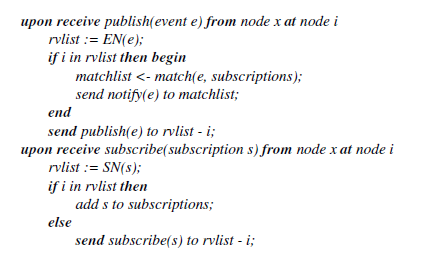
\includegraphics{6/Encuentro.png}
		\caption{Algoritmo de Encuentros. Tomado de \CO}
		\label{fig:encuentro}
	\end{figure}
	
\end{description}


%%%%%%%%%%%%%%%%%%%%%%%%%%%%%%%%%%%%%%%%%%%%%%%%%%%%%%%%%%%%%%

\section{Colas}
\label{sec:Colas}
\index{colas}


Mientras que los grupos y publicación-suscripción proporcionan un estilo de comunicación de uno a varios, las colas de mensajes proporcionan un servicio punto a punto utilizando el concepto de cola de mensajes como una indirección, logrando así las propiedades deseadas de desacoplamiento de espacio y tiempo. Son punto a punto en el sentido de que el remitente coloca el mensaje en una cola y luego es eliminado por un solo proceso. Las colas de mensajes también se conocen como \textit{Middleware orientado a mensajes.}

\subsection{Modelo de programación} \index{modelo de programaci\'on de colas}

El modelo de programación que ofrecen las colas de mensajes es muy sencillo. Ofrece un acercamiento a la comunicación en sistemas distribuidos a través de colas. En particular, los procesos productores pueden enviar mensajes a una cola específica y otros procesos (consumidores) pueden recibir mensajes de esta cola. Se admiten tres estilos de recepción:
\begin{itemize}
	\item una recepción con  bloqueo, que se bloqueará hasta que esté disponible un mensaje apropiado;
	\item una recepción sin bloqueo (una operación de sondeo), que verificará el estado de la cola y devolverá un mensaje si está disponible, o una indicación de no disponible en caso contrario;
	\item una operación de notificación, que emitirá una notificación de evento cuando un mensaje esté disponible en la cola asociada.
\end{itemize}

\begin{figure}
	\centering
	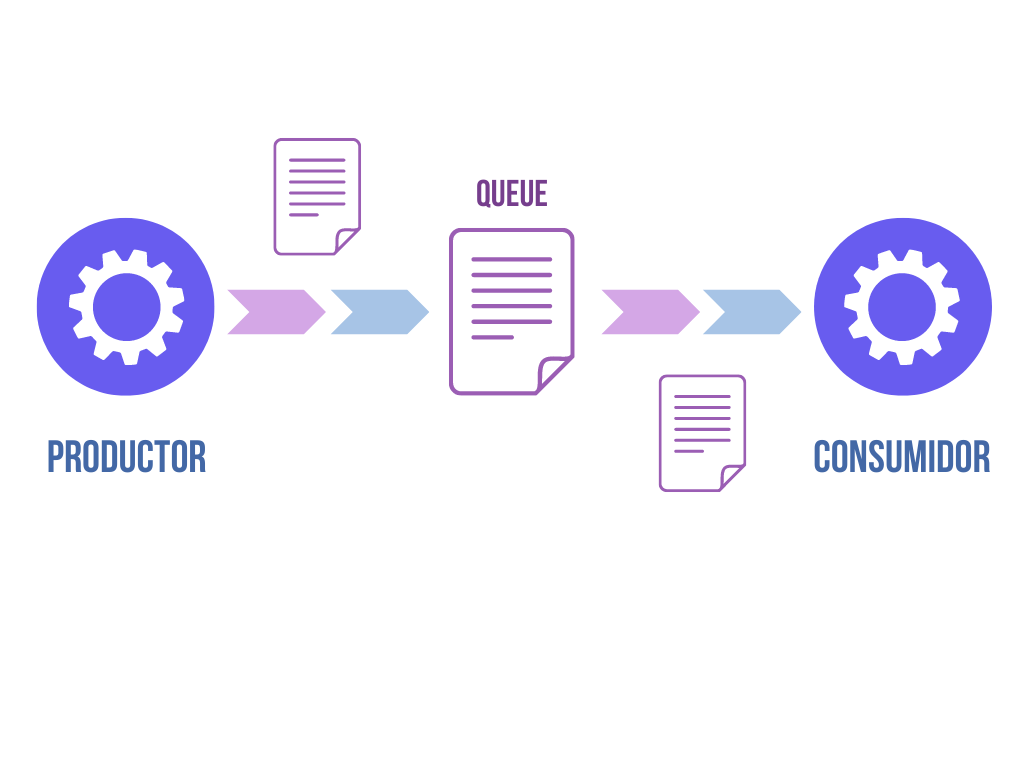
\includegraphics{6/7.png}
	\caption{Modelo de Programaci\'on.}
	\label{fig:cola}
\end{figure}

\subsection{Caracter\'isticas}
\index{caracter\'isticas de colas}
Entre sus caracter\'isticas:
\begin{itemize}
	\item Varios procesos pueden enviar mensajes a la misma cola y, del mismo modo, varios receptores pueden eliminar mensajes de una cola.
	\item La política de colas es  el primero en entrar, primero en salir (FIFO), pero la mayoría de las implementaciones de colas de mensajes también admiten el concepto de prioridad, con los mensajes de mayor prioridad entregados primero. Los procesos de consumidor también pueden seleccionar mensajes de la cola según las propiedades de un mensaje.
	\item Un mensaje consta de un destino ( un identificador único que designa la cola de destino), metadatos asociados con el mensaje, incluidos campos como la prioridad del mensaje y el modo de entrega, y también el cuerpo del mensaje.
	\item Los mensajes son persistentes, es decir, las colas de mensajes almacenarán los mensajes indefinidamente (hasta que se consuman) y también enviarán los mensajes al disco para permitir una entrega confiable.
	\item  Cualquier mensaje enviado se recibe eventualmente (validez) y el mensaje recibido es idéntico al enviado, y ningún mensaje se entrega dos veces (integridad). Por lo tanto, los sistemas de cola de mensajes garantizan que los mensajes se entregarán (y se entregarán una vez), pero no pueden decir nada sobre el momento de la entrega.
\end{itemize}

%%%%%%%%%%%%%%%%%%%%%%%%%%%%%%%%%%%%%%%%%%%%%%%%


\section{Casos de Estudio: Patr\'on y mensajer\'ia Pub/sub}
\label{ch:CasoEstudio}

\index{caso de estudio!patrón pub-sub} 
\index{caso de estudio!mensajer\'ia pub-sub} 

\subsection{Mensajer\'ia Publicaci\'on Suscripci\'on}
 


En arquitectura de software,\textbf{ Mensajer\'ia Pub/Sub}, también conocido como \textbf{patrón Pub/Sub} \sidecite{Singh2022}, es un patrón de mensajería que proporciona un marco para el intercambio de mensajes  en el que los remitentes de mensajes, llamados editores, no programan los mensajes para que se envíen directamente a receptores específicos, llamados suscriptores, sino que clasifican los mensajes publicados en clases sin saber qué suscriptores, si  los hay.
De igual forma, los suscriptores expresan interés en una o más clases de mensajes y solo reciben mensajes que son de su interés, sin saber qué editores, si los hay.


Los sistemas de Mensajer\'ia Pub/sub es un hermano del paradigma de la cola de mensajes y, por lo general, es una parte de un sistema de middleware orientado a mensajes. 
La Mensajer\'ia Pub/sub permite el acoplamiento flexible y la escala entre el remitente de mensajes (editores) y los receptores (suscriptores) en los agentes de mensajería a los que se suscriben. Algunas de las tecnologías comunes que utilizan Pub/Sub Messaging son RabbitMQ, Kafka, Redis, etc.

Los mensajes se envían desde un editor a los suscriptores a medida que están disponibles. Los editores son servicios que envían mensajes al intermediario de mensajes. Luego, los suscriptores se suscriben a los corredores de mensajes que les interesan para escuchar estos mensajes.

En la figura \ref{fig:patron} se muestra los componentes de este sistema.

\begin{figure}
	\centering
	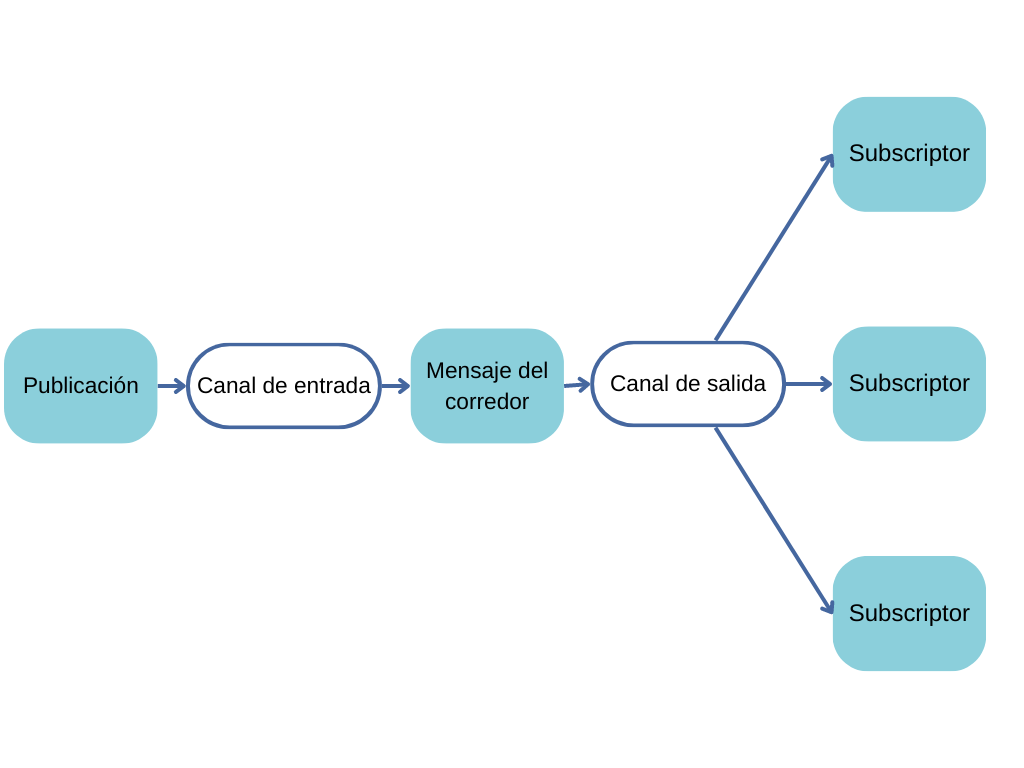
\includegraphics{6/mod-pubsub-mens.PNG}
	\caption{Patr\'on Publicaci\'on-Suscripci\'on.}
	\label{fig:patron}
\end{figure}

La mensajería de publicación/suscripción tiene los siguientes beneficios \sidecite{Azure2023}:

\begin{itemize}
	\item Acoplamiento bajo entre los componentes, lo que hace que su sistema sea más modular y flexible.
	
	\item 	Alta escalabilidad (en teoría, Pub/Sub permite que cualquier cantidad de editores se comunique con cualquier cantidad de suscriptores).
	
	\item Mejora la fiabilidad. La mensajería asincrónica ayuda a que las aplicaciones continúen funcionando sin problemas bajo cargas mayores y manejen fallas intermitentes de manera más efectiva
	
	\item Permite el procesamiento diferido o programado. Los suscriptores pueden esperar para recoger los mensajes hasta las horas de menor actividad, o los mensajes pueden enrutarse o procesarse de acuerdo con un cronograma específico.
	
	\item Permite una integración  entre sistemas que utilizan diferentes plataformas, lenguajes de programación o protocolos de comunicación, así como entre sistemas locales y aplicaciones que se ejecutan en la nube.
	
	\item Comunicación asincrónica basada en eventos que es ideal para aplicaciones de baja latencia en tiempo real.
	
	
\end{itemize}

%\marginnote[-2cm]{
	\begin{kaobox}[frametitle=Patrón Pub/Sub]
		
	
Lectura recomendada:
 \href{https://medium.com/frontend-canteen/publish-subscribe-pattern-in-javascript-17bf1e94e83d#id_token=eyJhbGciOiJSUzI1NiIsImtpZCI6IjgyMjgzOGMxYzhiZjllZGNmMWY1MDUwNjYyZTU0YmNiMWFkYjViNWYiLCJ0eXAiOiJKV1QifQ.eyJpc3MiOiJodHRwczovL2FjY291bnRzLmdvb2dsZS5jb20iLCJuYmYiOjE2ODQ1MTIzMjMsImF1ZCI6IjIxNjI5NjAzNTgzNC1rMWs2cWUwNjBzMnRwMmEyamFtNGxqZGNtczAwc3R0Zy5hcHBzLmdvb2dsZXVzZXJjb250ZW50LmNvbSIsInN1YiI6IjEwMjI2OTQwMjQ2Mjg2MzkwNDE1OCIsImVtYWlsIjoidmlyZ2luaWFwYWRpbGxhc0BnbWFpbC5jb20iLCJlbWFpbF92ZXJpZmllZCI6dHJ1ZSwiYXpwIjoiMjE2Mjk2MDM1ODM0LWsxazZxZTA2MHMydHAyYTJqYW00bGpkY21zMDBzdHRnLmFwcHMuZ29vZ2xldXNlcmNvbnRlbnQuY29tIiwibmFtZSI6IlZpcmdpbmlhIFBhZGlsbGEiLCJwaWN0dXJlIjoiaHR0cHM6Ly9saDMuZ29vZ2xldXNlcmNvbnRlbnQuY29tL2EvQUdObXl4YnlCQmtNU054M0lhdldhR3JyMlFFTGpZU0dkR2FoR3NGRG9MZV9MQT1zOTYtYyIsImdpdmVuX25hbWUiOiJWaXJnaW5pYSIsImZhbWlseV9uYW1lIjoiUGFkaWxsYSIsImlhdCI6MTY4NDUxMjYyMywiZXhwIjoxNjg0NTE2MjIzLCJqdGkiOiIxOTdiZjk4YTU5OGIwODM1MjVjN2RiNWM5MGMyNGYxZWIyNTU2OTZhIn0.jUHSvQ97J4DWJiKJM3z_cWvwhJaLt_kWAAapQG9b8W1e1t5KEg_z6FVGzV68N8gpEqGSF8KP7CElRyxJgQIGsaCooqXPkZ60l7ue0Yu4j6VC6gY2bnjmKi6jbIAR7trWa-ahRa0U9g3Ss1MNw_8cppiM3jpkgjjvY_WE91J__VEUC9Z2vov7aQoCNQk0kR9uCXnXVFkiAD0EIESD_rWWhjgvlLwenBgF8wy2DhzsUsHCBVxfRwdYiGibVwFdQZuI9hxSLboH9Af4p1X1EAV9tThxQb6tdQs1xjQVWVbmTjSoMUeHwH0-MV7ZeTctf0O5QGYRpuRqOhvzdZnGYHddTQ}{Publish-Subscribe Pattern: The Most Used Patterns in JavaScript}

	\end{kaobox} 

\subsection{Rabbit MQ}

\textbf{RabbitMQ} es un software de intermediario (broker o corredores) de mensajes de código abierto (a veces llamado middleware orientado a mensajes) que originalmente implementó el Protocolo de cola de mensajes avanzado (AMQP) y desde entonces se ha ampliado con una arquitectura   para admitir el Protocolo de mensajería orientada a texto en streaming (\textbf{STOMP}), MQ Telemetry Transport (\textbf{MQTT}) y otros protocolos.

Escrito en \textbf{Erlang} , el servidor RabbitMQ se basa en el marco de Open Telecom Platform para la agrupación en clústeres y la conmutación por error. Las bibliotecas de cliente para interactuar con el intermediario están disponibles para los principales lenguajes de programación. El código fuente se publica bajo la licencia pública de Mozilla.


\begin{kaobox}[frametitle=Erlang]
	Erlang es un lenguaje de programación que se utiliza para construir sistemas de software en tiempo real escalables masivamente con requisitos de alta disponibilidad. Algunos de sus usos se encuentran en telecomunicaciones, banca, comercio electrónico, telefonía informática y mensajería instantánea.  
	M\'as de \href{https://www.erlang.org/}{Elang} en esa direcci\'on. 
\end{kaobox}



%\marginnote[-4.2cm]{
	\begin{kaobox}[frametitle=Rabbit MQ]
		
		Conozca acerca de este tema en \href{https://blog.bi-geek.com/rabbitmq-para-principiantes/}{Rabbit MQ}
		
	\end{kaobox}   

